% Convert with command:
% convert -density 300 pic.pdf -quality 90 pic.png
\documentclass[crop,tikz,border=0pt]{standalone}
\usetikzlibrary{arrows.meta, fit}
\begin{document}

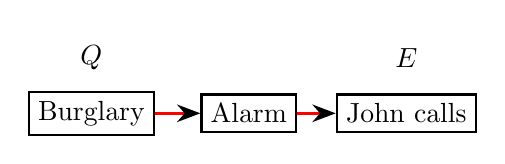
\begin{tikzpicture}
\begin{scope}[every node/.style={circle,thick,draw}]
    \node (burglary) at (0, 0) [shape=rectangle, fill=white] {Burglary};
    \node (btext) at (0, 0.7) [shape=circle,draw=white,fill=white] {$Q$};

    \node (alarm) at (2, 0) [shape=rectangle, fill=white] {Alarm};

    \node (john) at (4, 0) [shape=rectangle, fill=white] {John calls};
    \node (jtext) at (4, 0.7) [shape=circle,draw=white,fill=white] {$E$};
\end{scope}

\begin{scope}[>={Stealth[black]},
            %   every node/.style={fill=white,rectangle,above},
              every edge/.style={draw=red,very thick}]
    \path [->] (burglary) edge node {} (alarm);
    \path [->] (alarm) edge node {} (john);
\end{scope}
\end{tikzpicture}

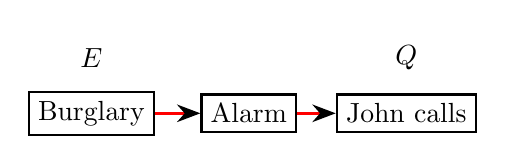
\begin{tikzpicture}
\begin{scope}[every node/.style={circle,thick,draw}]
    \node (burglary) at (0, 0) [shape=rectangle, fill=white] {Burglary};
    \node (btext) at (0, 0.7) [shape=circle,draw=white,fill=white] {$E$};

    \node (alarm) at (2, 0) [shape=rectangle, fill=white] {Alarm};

    \node (john) at (4, 0) [shape=rectangle, fill=white] {John calls};
    \node (jtext) at (4, 0.7) [shape=circle,draw=white,fill=white] {$Q$};
\end{scope}

\begin{scope}[>={Stealth[black]},
            %   every node/.style={fill=white,rectangle,above},
              every edge/.style={draw=red,very thick}]
    \path [->] (burglary) edge node {} (alarm);
    \path [->] (alarm) edge node {} (john);
\end{scope}
\end{tikzpicture}

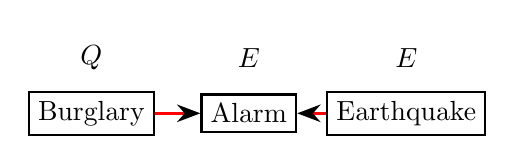
\begin{tikzpicture}
\begin{scope}[every node/.style={circle,thick,draw}]
    \node (burglary) at (0, 0) [shape=rectangle, fill=white] {Burglary};
    \node (btext) at (0, 0.7) [shape=circle,draw=white,fill=white] {$Q$};

    \node (alarm) at (2, 0) [shape=rectangle, fill=white] {Alarm};
    \node (etext1) at (2, 0.7) [shape=circle,draw=white,fill=white] {$E$};

    \node (earthquake) at (4, 0) [shape=rectangle, fill=white] {Earthquake};
    \node (etext2) at (4, 0.7) [shape=circle,draw=white,fill=white] {$E$};
\end{scope}

\begin{scope}[>={Stealth[black]},
            %   every node/.style={fill=white,rectangle,above},
              every edge/.style={draw=red,very thick}]
    \path [->] (burglary) edge node {} (alarm);
    \path [->] (earthquake) edge node {} (alarm);
\end{scope}
\end{tikzpicture}

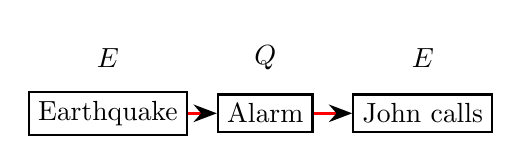
\begin{tikzpicture}
\begin{scope}[every node/.style={circle,thick,draw}]
    \node (earthquake) at (0, 0) [shape=rectangle, fill=white] {Earthquake};
    \node (btext) at (0, 0.7) [shape=circle,draw=white,fill=white] {$E$};

    \node (alarm) at (2, 0) [shape=rectangle, fill=white] {Alarm};
    \node (etext1) at (2, 0.7) [shape=circle,draw=white,fill=white] {$Q$};

    \node (john) at (4, 0) [shape=rectangle, fill=white] {John calls};
    \node (etext2) at (4, 0.7) [shape=circle,draw=white,fill=white] {$E$};
\end{scope}

\begin{scope}[>={Stealth[black]},
            %   every node/.style={fill=white,rectangle,above},
              every edge/.style={draw=red,very thick}]
    \path [->] (earthquake) edge node {} (alarm);
    \path [->] (alarm) edge node {} (john);
\end{scope}
\end{tikzpicture}

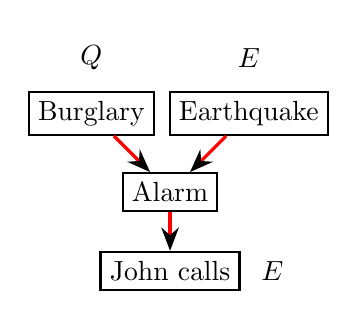
\begin{tikzpicture}
\begin{scope}[every node/.style={circle,thick,draw}]
    \node (burglary) at (0, 0) [shape=rectangle, fill=white] {Burglary};
    \node (btext) at (0, 0.7) [shape=circle,draw=white,fill=white] {$Q$};

    \node (earthquake) at (2, 0) [shape=rectangle, fill=white] {Earthquake};
    \node (etext1) at (2, 0.7) [shape=circle,draw=white,fill=white] {$E$};

    \node (alarm) at (1, -1) [shape=rectangle, fill=white] {Alarm};

    \node (john) at (1, -2) [shape=rectangle, fill=white] {John calls};
    \node (etext2) at (2.3, -2) [shape=circle,draw=white,fill=white] {$E$};
\end{scope}

\begin{scope}[>={Stealth[black]},
            %   every node/.style={fill=white,rectangle,above},
              every edge/.style={draw=red,very thick}]
    \path [->] (burglary) edge node {} (alarm);
    \path [->] (earthquake) edge node {} (alarm);
    \path [->] (alarm) edge node {} (john);
\end{scope}
\end{tikzpicture}
\end{document}
